\documentclass{article}
    
\usepackage{tkz-tab}

\begin{document}
DONNER LES VARIATIONS DE f(x)\\

$f(x)=- x^{5} - x^{4} + x^{3} + x^{2}$\\
$f'(x)= - 5 x^{4} - 4 x^{3} + 3 x^{2} + 2 x$\\

    

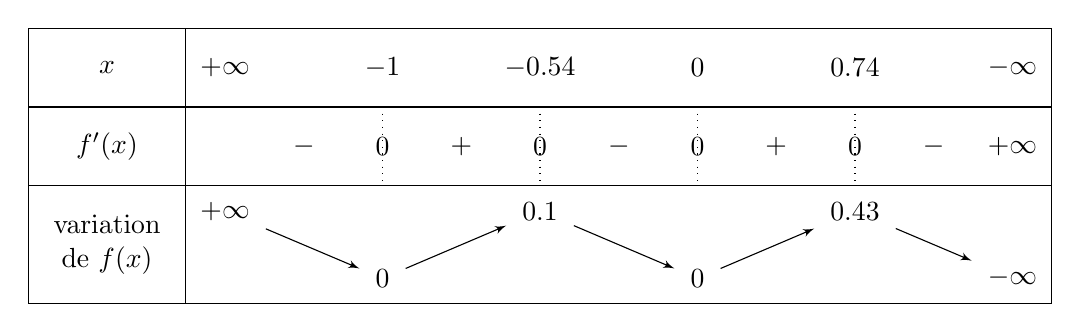
\begin{tikzpicture}

   \tkzTabInit[espcl=2]{$x$ / 1 , $f'(x)$ / 1, variation de $f(x)$/1.5}
   {$+\infty$, $-1$,$-0.54$,$0$,$0.74$,$-\infty$}

   \tkzTabLine{,-,z,+,z,-,z,+,z,-,+\infty}
   \tkzTabVar{+/$+\infty$,-/$0$,+/$0.1$,-/$0$,+/$0.43$,-/$-\infty$}



\end{tikzpicture}


\end{document}
